\subsection{Removing strategy hints from unchanged problems}

\label{sec:prompt-hint-ablation}

We freeze a paired follow-up on Python factors, MathIR, and Pantry at Levels 2 and 3. Within each of these six cells, the 32 smallest SHA-256 hashes of $(20260911,\mathrm{level},\mathrm{domain},\mathrm{row\ index})$ select problems from the 128-row evaluation split, without consulting outcomes. Both arms generate eight fresh draws per identical problem. The original arm retains the published prompt. The neutral arm removes the Python suggestions to test small divisors with nested conditionals or dispatch on listed values, the MathIR ordered algebraic-isolation suggestion, and the Pantry preference for high-energy/protein, low-sodium ingredients such as seeds or oats. MathIR changes ``those operations to ``the operations to preserve the menu-ID instruction. The user problem, answer specification, executable verifier, and remaining format requirements are unchanged.

We report the paired neutral-minus-original effects on empirical $P_8=\texttt{pass@8}$ and $D_8=\texttt{distinct@8}$, with $B_8=D_8-P_8$ as additional verified breadth. All returned answers, including incorrect, empty, and truncated outputs, remain in their eight-draw groups; only verifier-accepted outputs create a verified key. Strict verification is primary; one unchanged, previously frozen formatting normalizer is a sensitivity analysis and preserves every strict success and canonical key. Python outputs in both arms undergo the same serial, warmed-verifier recheck, with original grades and any corrections retained in separate receipts.

Intervals use 20,000 whole-prompt bootstrap resamples, paired across arms and stratified by domain and level (seed 20260911). Cells contribute equally to reported macros. These are pointwise exploratory intervals for 32 problems per cell; crossing zero does not establish equivalence or absence of a prompt effect. A zero-width bootstrap interval records zero observed resampled variation, including all-tied $P_8$ outcomes; it is not precise evidence of population equivalence. Correct-pair collision and the certified-support uniform reference are secondary and retain their correct-pair denominators; the machine-readable report includes joint eligibility counts and undefined cells. Eight sampled draws do not identify total unseen support.



This appendix reports the complete local panel only. The separately registered frontier panel is not included here, and the overall local-plus-frontier experiment is incomplete.

For local models, we evaluate the initial Qwen2.5-0.5B model and fixed Level-2-trained DrGRPO and Replay DrGRPO checkpoints. Python and MathIR use matched training seeds 43--47; Pantry uses seeds 43 and 46. Level 3 is transfer evaluation. Seed means retain the same selected problem set across checkpoints. Five-seed intervals resample whole training seeds and paired prompts; Pantry reports both seed effects and intervals conditional on the two checkpoints. The native local syntax constraints and 192-token budget differ from hosted inference, so effects are interpreted within each model and interface.


\begin{table}[t]
\centering
\scriptsize
\setlength{\tabcolsep}{3pt}
\caption{Local Qwen2.5-0.5B checkpoints under strict verification. Each arrow gives original $\to$ neutral. $P_8$ is empirical \texttt{pass@8}, $D_8$ is verified \texttt{distinct@8}, and $B_8=D_8-P_8$. Effects are neutral minus original; brackets are pointwise 95\% intervals. Local rows average the displayed number of training seeds. Five-seed intervals include seed and paired-prompt resampling; two-seed Pantry intervals condition on the two fixed checkpoints. }
\label{tab:prompt-hints-local-strict}
\begin{tabular}{llrrrrr}
\toprule
Model & Cell & $P_8$: O$\to$N & $D_8$: O$\to$N & $\Delta P_8$ [95\%] & $\Delta D_8$ [95\%] & $\Delta B_8$ \\
\midrule
Initial Qwen 0.5B ($s=1$) & Python factors L2 & $0.656\to0.125$ & $0.69\to0.12$ & $-0.531\;[-0.719,-0.344]$ & $-0.56\;[-0.75,-0.38]$ & $-0.03$ \\
Initial Qwen 0.5B ($s=1$) & MathIR L2 & $0.250\to0.281$ & $0.25\to0.28$ & $+0.031\;[+0.000,+0.094]$ & $+0.03\;[+0.00,+0.09]$ & $+0.00$ \\
Initial Qwen 0.5B ($s=1$) & Pantry L2 & $0.156\to0.188$ & $0.19\to0.22$ & $+0.031\;[+0.000,+0.094]$ & $+0.03\;[+0.00,+0.09]$ & $+0.00$ \\
Initial Qwen 0.5B ($s=1$) & Python factors L3 & $0.719\to0.031$ & $0.81\to0.03$ & $-0.688\;[-0.844,-0.531]$ & $-0.78\;[-0.97,-0.59]$ & $-0.09$ \\
Initial Qwen 0.5B ($s=1$) & MathIR L3 & $0.219\to0.219$ & $0.22\to0.22$ & $+0.000\;[-0.125,+0.125]$ & $+0.00\;[-0.12,+0.12]$ & $+0.00$ \\
Initial Qwen 0.5B ($s=1$) & Pantry L3 & $0.281\to0.312$ & $0.66\to0.69$ & $+0.031\;[+0.000,+0.094]$ & $+0.03\;[-0.06,+0.12]$ & $+0.00$ \\
DrGRPO ($s=5$) & MathIR L2 & $0.531\to0.506$ & $0.53\to0.51$ & $-0.025\;[-0.100,+0.031]$ & $-0.03\;[-0.10,+0.03]$ & $+0.00$ \\
DrGRPO ($s=5$) & MathIR L3 & $0.194\to0.156$ & $0.19\to0.16$ & $-0.037\;[-0.113,+0.019]$ & $-0.04\;[-0.11,+0.02]$ & $+0.00$ \\
DrGRPO ($s=2$) & Pantry L2 & $0.219\to0.203$ & $0.28\to0.25$ & $-0.016\;[-0.156,+0.125]$ & $-0.03\;[-0.19,+0.12]$ & $-0.02$ \\
DrGRPO ($s=2$) & Pantry L3 & $0.172\to0.172$ & $0.27\to0.25$ & $+0.000\;[-0.078,+0.078]$ & $-0.02\;[-0.16,+0.11]$ & $-0.02$ \\
DrGRPO ($s=5$) & Python factors L2 & $0.812\to0.000$ & $0.81\to0.00$ & $-0.812\;[-0.938,-0.656]$ & $-0.81\;[-0.94,-0.66]$ & $+0.00$ \\
DrGRPO ($s=5$) & Python factors L3 & $1.000\to0.000$ & $1.00\to0.00$ & $-1.000\;[-1.000,-1.000]$ & $-1.00\;[-1.00,-1.00]$ & $+0.00$ \\
Replay DrGRPO ($s=5$) & MathIR L2 & $0.994\to0.975$ & $0.99\to0.97$ & $-0.019\;[-0.075,+0.000]$ & $-0.02\;[-0.07,+0.00]$ & $+0.00$ \\
Replay DrGRPO ($s=5$) & MathIR L3 & $0.312\to0.275$ & $0.31\to0.28$ & $-0.037\;[-0.138,+0.044]$ & $-0.04\;[-0.14,+0.04]$ & $+0.00$ \\
Replay DrGRPO ($s=2$) & Pantry L2 & $0.516\to0.500$ & $0.75\to0.73$ & $-0.016\;[-0.109,+0.078]$ & $-0.02\;[-0.20,+0.17]$ & $+0.00$ \\
Replay DrGRPO ($s=2$) & Pantry L3 & $0.234\to0.281$ & $0.39\to0.50$ & $+0.047\;[+0.000,+0.109]$ & $+0.11\;[+0.05,+0.19]$ & $+0.06$ \\
Replay DrGRPO ($s=5$) & Python factors L2 & $0.887\to0.556$ & $1.24\to0.68$ & $-0.331\;[-0.525,-0.150]$ & $-0.57\;[-0.85,-0.32]$ & $-0.24$ \\
Replay DrGRPO ($s=5$) & Python factors L3 & $1.000\to0.494$ & $1.42\to0.66$ & $-0.506\;[-0.825,-0.194]$ & $-0.76\;[-1.07,-0.38]$ & $-0.26$ \\
\bottomrule
\end{tabular}
\end{table}


\begin{table}[t]
\centering
\scriptsize
\setlength{\tabcolsep}{3pt}
\caption{Local Qwen2.5-0.5B checkpoints under frozen formatting normalization. Each arrow gives original $\to$ neutral. $P_8$ is empirical \texttt{pass@8}, $D_8$ is verified \texttt{distinct@8}, and $B_8=D_8-P_8$. Effects are neutral minus original; brackets are pointwise 95\% intervals. Local rows average the displayed number of training seeds. Five-seed intervals include seed and paired-prompt resampling; two-seed Pantry intervals condition on the two fixed checkpoints. }
\label{tab:prompt-hints-local-normalized-secondary}
\begin{tabular}{llrrrrr}
\toprule
Model & Cell & $P_8$: O$\to$N & $D_8$: O$\to$N & $\Delta P_8$ [95\%] & $\Delta D_8$ [95\%] & $\Delta B_8$ \\
\midrule
Initial Qwen 0.5B ($s=1$) & Python factors L2 & $0.656\to0.125$ & $0.69\to0.12$ & $-0.531\;[-0.719,-0.344]$ & $-0.56\;[-0.75,-0.38]$ & $-0.03$ \\
Initial Qwen 0.5B ($s=1$) & MathIR L2 & $0.250\to0.281$ & $0.25\to0.28$ & $+0.031\;[+0.000,+0.094]$ & $+0.03\;[+0.00,+0.09]$ & $+0.00$ \\
Initial Qwen 0.5B ($s=1$) & Pantry L2 & $0.156\to0.188$ & $0.19\to0.22$ & $+0.031\;[+0.000,+0.094]$ & $+0.03\;[+0.00,+0.09]$ & $+0.00$ \\
Initial Qwen 0.5B ($s=1$) & Python factors L3 & $0.719\to0.031$ & $0.81\to0.03$ & $-0.688\;[-0.844,-0.531]$ & $-0.78\;[-0.97,-0.59]$ & $-0.09$ \\
Initial Qwen 0.5B ($s=1$) & MathIR L3 & $0.219\to0.219$ & $0.22\to0.22$ & $+0.000\;[-0.125,+0.125]$ & $+0.00\;[-0.12,+0.12]$ & $+0.00$ \\
Initial Qwen 0.5B ($s=1$) & Pantry L3 & $0.281\to0.312$ & $0.66\to0.69$ & $+0.031\;[+0.000,+0.094]$ & $+0.03\;[-0.06,+0.12]$ & $+0.00$ \\
DrGRPO ($s=5$) & MathIR L2 & $0.531\to0.506$ & $0.53\to0.51$ & $-0.025\;[-0.100,+0.031]$ & $-0.03\;[-0.10,+0.03]$ & $+0.00$ \\
DrGRPO ($s=5$) & MathIR L3 & $0.194\to0.156$ & $0.19\to0.16$ & $-0.037\;[-0.113,+0.019]$ & $-0.04\;[-0.11,+0.02]$ & $+0.00$ \\
DrGRPO ($s=2$) & Pantry L2 & $0.219\to0.203$ & $0.28\to0.25$ & $-0.016\;[-0.156,+0.125]$ & $-0.03\;[-0.19,+0.12]$ & $-0.02$ \\
DrGRPO ($s=2$) & Pantry L3 & $0.172\to0.172$ & $0.27\to0.25$ & $+0.000\;[-0.078,+0.078]$ & $-0.02\;[-0.16,+0.11]$ & $-0.02$ \\
DrGRPO ($s=5$) & Python factors L2 & $0.812\to0.000$ & $0.81\to0.00$ & $-0.812\;[-0.938,-0.656]$ & $-0.81\;[-0.94,-0.66]$ & $+0.00$ \\
DrGRPO ($s=5$) & Python factors L3 & $1.000\to0.000$ & $1.00\to0.00$ & $-1.000\;[-1.000,-1.000]$ & $-1.00\;[-1.00,-1.00]$ & $+0.00$ \\
Replay DrGRPO ($s=5$) & MathIR L2 & $0.994\to0.975$ & $0.99\to0.97$ & $-0.019\;[-0.075,+0.000]$ & $-0.02\;[-0.07,+0.00]$ & $+0.00$ \\
Replay DrGRPO ($s=5$) & MathIR L3 & $0.312\to0.275$ & $0.31\to0.28$ & $-0.037\;[-0.138,+0.044]$ & $-0.04\;[-0.14,+0.04]$ & $+0.00$ \\
Replay DrGRPO ($s=2$) & Pantry L2 & $0.516\to0.500$ & $0.75\to0.73$ & $-0.016\;[-0.109,+0.078]$ & $-0.02\;[-0.20,+0.17]$ & $+0.00$ \\
Replay DrGRPO ($s=2$) & Pantry L3 & $0.234\to0.281$ & $0.39\to0.50$ & $+0.047\;[+0.000,+0.109]$ & $+0.11\;[+0.05,+0.19]$ & $+0.06$ \\
Replay DrGRPO ($s=5$) & Python factors L2 & $0.887\to0.556$ & $1.24\to0.68$ & $-0.331\;[-0.525,-0.150]$ & $-0.57\;[-0.85,-0.32]$ & $-0.24$ \\
Replay DrGRPO ($s=5$) & Python factors L3 & $1.000\to0.494$ & $1.42\to0.66$ & $-0.506\;[-0.825,-0.194]$ & $-0.76\;[-1.07,-0.38]$ & $-0.26$ \\
\bottomrule
\end{tabular}
\end{table}


\begin{figure}[t]

\centering

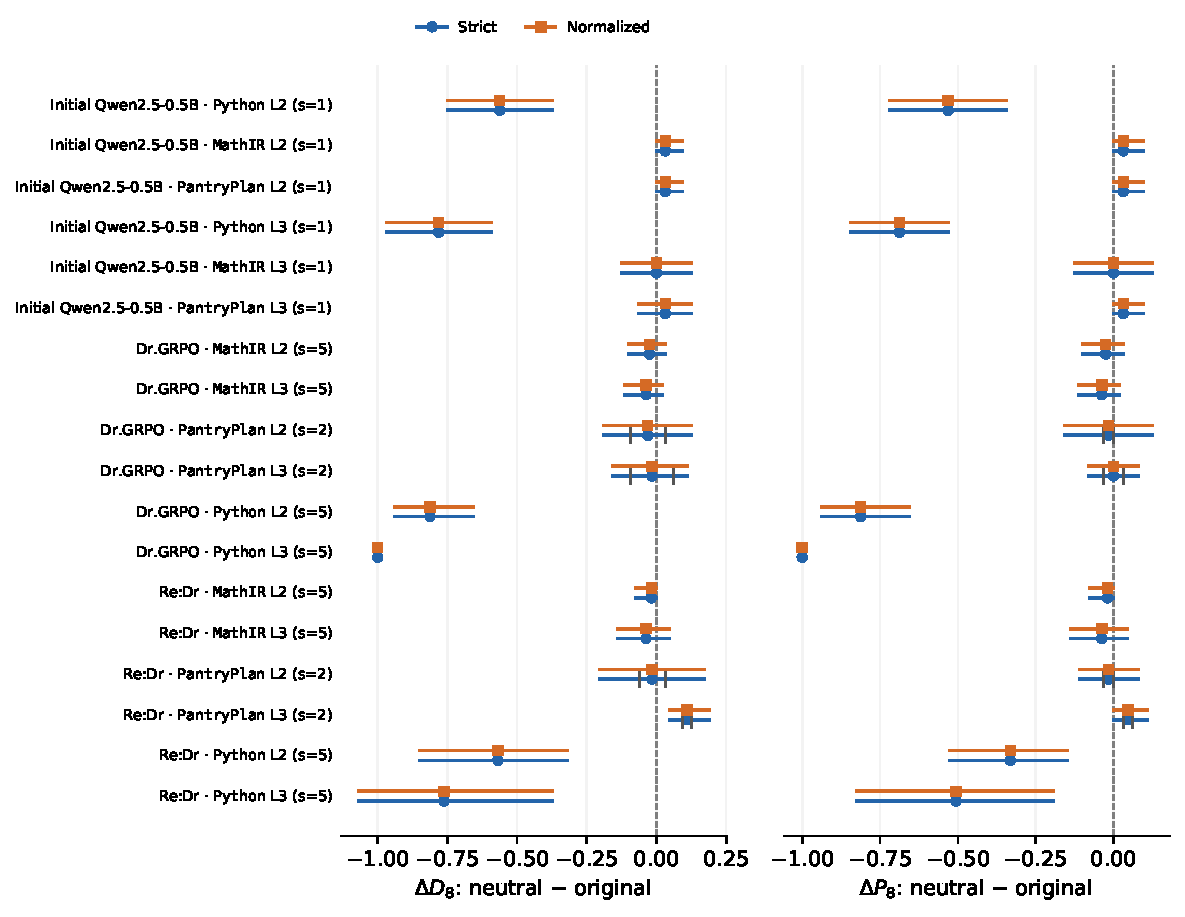
\includegraphics[width=\linewidth]{figures/modebench_prompt_ablation_local.pdf}

\caption{Prompt-hint removal effects for local checkpoints, preserving every registered domain--level cell. Blue circles use strict verification; orange squares use the same frozen formatting normalizer. Horizontal bars show the intervals described in the tables; zero is the vertical reference. Gray endpoint marks show the two individual Pantry seed effects. }

\label{fig:prompt-hints-local}

\end{figure}



\paragraph{Two-seed Pantry sensitivity.} Two checkpoints cannot support a stable estimate of training-seed variability. The following lists both strict prompt effects; the intervals in the local table condition on these two checkpoints.
DrGRPO L2 (seed 43: $\Delta P_8=+0.000$, $\Delta D_8=+0.03$; seed 46: $\Delta P_8=-0.031$, $\Delta D_8=-0.09$); DrGRPO L3 (seed 43: $\Delta P_8=+0.031$, $\Delta D_8=+0.06$; seed 46: $\Delta P_8=-0.031$, $\Delta D_8=-0.09$); Replay DrGRPO L2 (seed 43: $\Delta P_8=-0.031$, $\Delta D_8=-0.06$; seed 46: $\Delta P_8=+0.000$, $\Delta D_8=+0.03$); Replay DrGRPO L3 (seed 43: $\Delta P_8=+0.031$, $\Delta D_8=+0.12$; seed 46: $\Delta P_8=+0.062$, $\Delta D_8=+0.09$).
